\label{ch:experimental_techniques}

\section{LIBS}
\label{sec:LIBS}
Laser-Induced Breakdown Spectroscopy (LIBS) is an atomic emission spectroscopy technique that utilizes high energy laser pulses to create plasma on the surface of material samples. It is a promising method in analytical chemistry and material analysis because it allows for the direct analysis of solid, liquid and even gas samples, without requiring any chemical preparation.
\\
The interaction between focused laser pulses and the sample leads to the creation of a plasma composed of ionized matter. This plasma emission can yield spectral signatures indicative of the chemical composition of various materials, regardless of their state of matter [Source: Fundamentals and Applications].
\\
LIBS offers the capability of conducting both qualitative and accurate quantitative analyses. Qualitative analysis involves discriminating between different components of a target sample, whereas quantitative analysis goes further by not only identifying the chemical components but also determining their relative concentrations.
\\
However, due to the modest repeatability of the method, attributed to the high variability present between each experiment [Source: Applications of single-shot laser], LIBS does not enable researchers to achieve detection limits and precision as low as those attainable with other methods. Consequently, it is primarily utilized for qualitative, semi-quantitative, or comparative analysis.
\\
The promising performance of this spectroscopy technique as a quantitative chemical analysis system has been facilitated by the development of new spectral processing algorithms in the last decade. These advancements have significantly broadened the application fields of LIBS. Today, LIBS finds applications ranging from diagnostics of archaeological objects to remote material assessment in nuclear power plants, and from the analysis of metal diffusion in solar cells to geological analysis in space explorations.

\subsection{LIBS technique}
\label{subsec:LIBS_technique}
The processes involved in LIBS include laser-sample interaction, material removal, breakdown process, and element-specific emission.
\\
Initially, the interaction between focused laser pulses and the target sample leads to the vaporization of a specific part of the surface area as the temperature reaches the sample material’s boiling point. The evaporated material forms a plume above the sample surface, and due to the continuous energy absorption of the laser, can result in the generation of a high-temperature plasma that will expand and eventually cool down.
[Analytical Chemistry LIBS]

\begin{figure}[H]
    \centering
    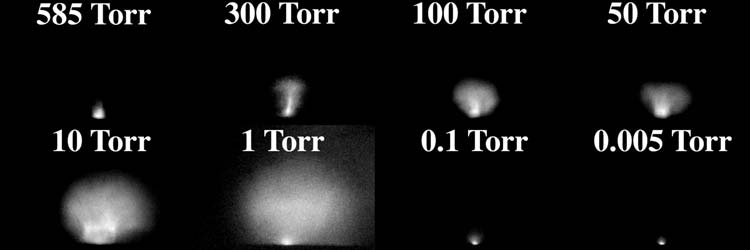
\includegraphics[width = 0.8\textwidth]{chapter_1/plasma_expansion_photo.png}
    \caption[Photo of a plasma expanding.]{ Change in the dimensions of a laser plasma as the air pressure was reduced.}
    \label{fig:plasma_expansion}
\end{figure}
[PHOTO TAKEN FROM LIBS: FUNDAMENTALS AND APPLICATIONS]

The light emitted from the plasma is indicative of the chemical composition of various materials. Positive identification of multiple elemental lines, including both wavelength and intensity within the emission spectrum, contributes to forming a unique spectral fingerprint of the target material. [Fundamentals and applications]
\\
The primary processes that occur during LIBS can be outlined in the following steps:

\begin{enumerate}
\item A short laser pulse is focused on the target material.
\item The incident optical energy is deposited on the sample, resulting in the vaporization of a small amount of its surface.
\item The incoming laser pulse, if its duration is sufficiently large, will also interact with the vapor plume to generate a high-temperature plasma.
\item The system employs a lens or an optical fiber to collect the light emitted from the plasma.
\item A dispersing device, such as a diffraction grating, spatially separates the emitted light into its components. This light originates from the spontaneous emission of hot atoms/ions in the plasma.
\item A digital sensor, such as a CCD or a PMT, is used to collect the light and generate the spectrum.
\item The wavelength and intensity of the resulting atomic emission peaks are analyzed to determine both the chemical elements present in the target sample and their relative concentrations.
\end{enumerate}
Each firing of the laser produces a single LIBS measurement. Typically, however, the signals from many laser plasmas are added or averaged to increase accuracy and precision and to average out nonconformities in sample composition. [LIBS Cambridge]

\begin{figure}[H]
    \centering
    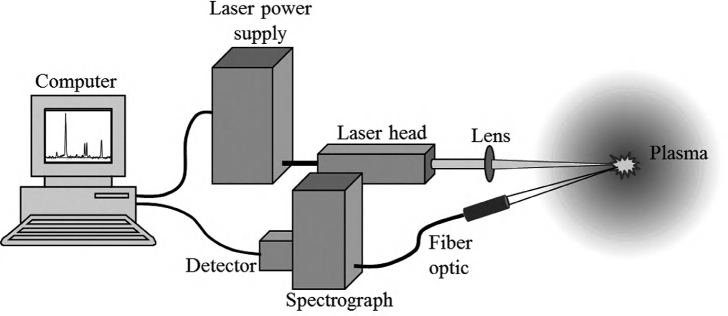
\includegraphics[width = \textwidth]{chapter_1/libs_setup.jpg}
    \caption{A schematic of a general apparatus for laser-induced breakdown spectroscopy illustrating the principal components.}
    \label{fig:libs_setup}
\end{figure}
[PHOTO TAKEN FROM HANDBOOK OF LIBS]

\subsection{Laser-sample Interaction}
\label{subsec:laser-sample_int}

When an atom absorbs a photon, it enters an excited state, where one of its electrons is promoted to a higher energy level. However, the excited states are not very stable, and electrons tend to transition to lower unpopulated energy levels either radiatively, when a photon is generated during the deexcitation process, and non-radiatively when the energy is dissipated in other forms, such as heat or vibration.
\\
Additionally, if the energy applied to the atom is sufficiently high to overcome the ionization potential, electrons can be detached from the atom, creating free negatively charged particles (electrons) and positively charged ions (cations). Initially, the outermost electron, with the lowest ionization potential, is the first to be detached. However, if the supplied energy is high enough, subsequent ionization potentials can be overcome, leading to the detachment of other electrons closer to the nucleus.
\\
There are two main steps leading to breakdown due to optical excitation. The first involves generating a few free electrons that serve as initial receptors of energy through collisions with photons and neutrals. The second is avalanche ionization in the focal region. Free electrons are accelerated by the electric field of the photons, and as the kinetic energy of the electrons grows, collisions will lead to further ionization that will generate even more electrons, creating an avalanche of ionization. 
\\
When a high-energy laser pulse is focused on the surface of a sample, if the irradiance at the focal point exceeds a certain threshold, atoms and ions are ejected from the surface in a process called ablation.

\begin{figure}[H]
    \centering
    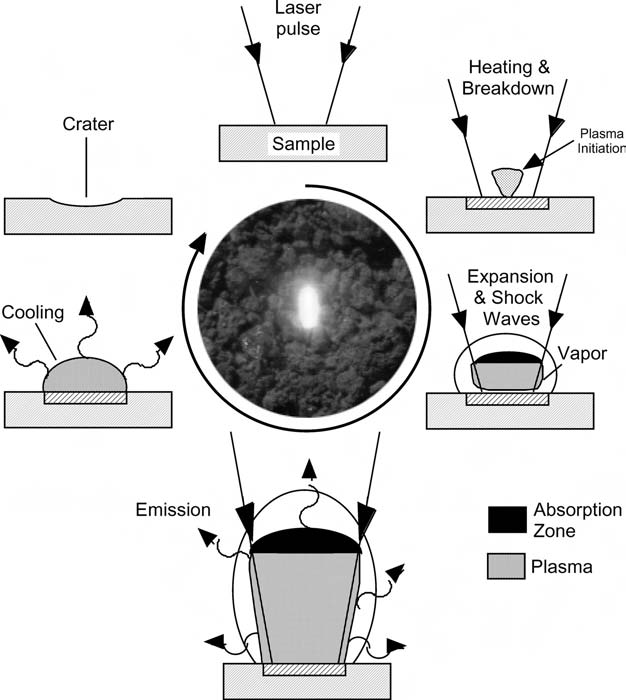
\includegraphics[width = 0.6\textwidth]{chapter_1/libs_life_cycle.png}
    \caption[LIBS life cycle.]{ Life cycle diagram showing main events in the LIBS process.}
    \label{fig:libs_life_cycle}
\end{figure}
[PHOTO TAKEN FROM Fundamentals and Applications]

\subsection{Plasma in LIBS}
\label{subsec:plasma_in_libs}
Given the numerous physical and chemical variables characterizing this state, various definitions of plasma are possible. A plasma can be defined as a local assembly of atoms, ions, molecules, and free electrons, that are overall electrically neutral and exhibit a collective behavior.
\\
Under typical conditions, such as atmospheric pressure and temperature, gases are primarily neutral, with only a marginable amount of charged particles. However, at high temperatures ($T > 1000K$), thermal dissociation of atoms and molecules occurs. Plasma forms when the average kinetic energy of the electrons (given by $k_bT$), significantly surpasses the average binding energy of an electron in an ion.
\\
Plasmas are characterized by a variety of parameters, such as the degree of ionization, the plasma temperature, and the electron density. Depending on the degree of ionization a plasma can be categorized as “weakly ionized”, where the ratio between electrons and other species is less than 10\%, or as “highly ionized” where, on the other hand, atoms could be stripped of many electrons, resulting in a very high electrons-to-ions ratio. LIBS plasmas typically fall in the first category of weakly ionized plasmas; in Figure~\ref{fig:plasma_parameters} we can see how LIBS plasmas compare in temperature and electron density relative to other types of plasma.
\begin{figure}[H]
    \centering
    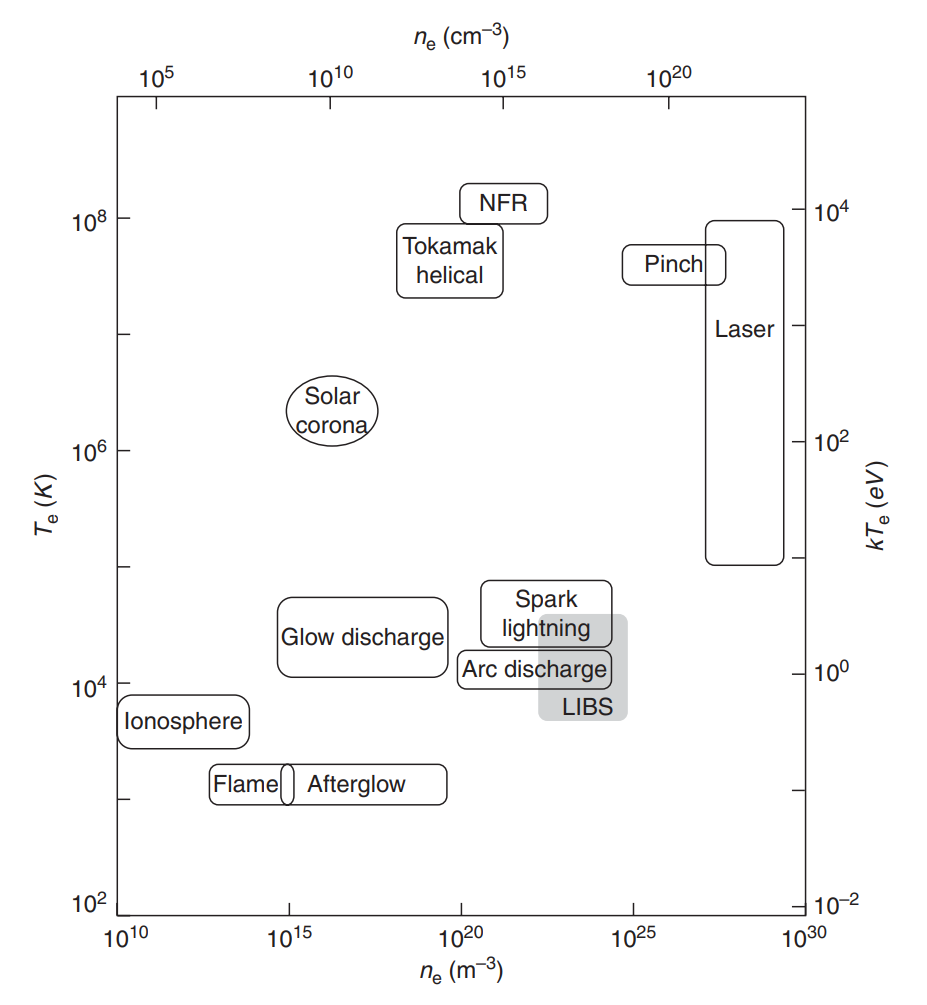
\includegraphics[width = 0.7\textwidth]{chapter_1/plasma_parameters.png}
    \caption{Relation between plasma parameters and type of plasma.}
    \label{fig:plasma_parameters}
\end{figure}
[PHOTO TAKEN FROM HANDBOOK OF LIBS]
The characteristics of the radiation emitted by the plasma depend on the type of radiative transitions that are occurring. At earlier times, where the plasma ionization level is high, the emission will be dominated by a continuum produced by both the bremsstrahlung (free-free transition) and the recombination processes (free-bound transition). Recombination occurs when a free electron is captured by a free ion, releasing its kinetic energy radiatively; while in bremsstrahlung the light is emitted due to electrons being accelerated or decelerated in collisions.
\\
However, the most interesting emissions that can be used for elemental analysis are caused by bound-to-bound transitions that occur between energy levels of ions, atoms, and molecules. 
\begin{figure}[H]
    \centering
    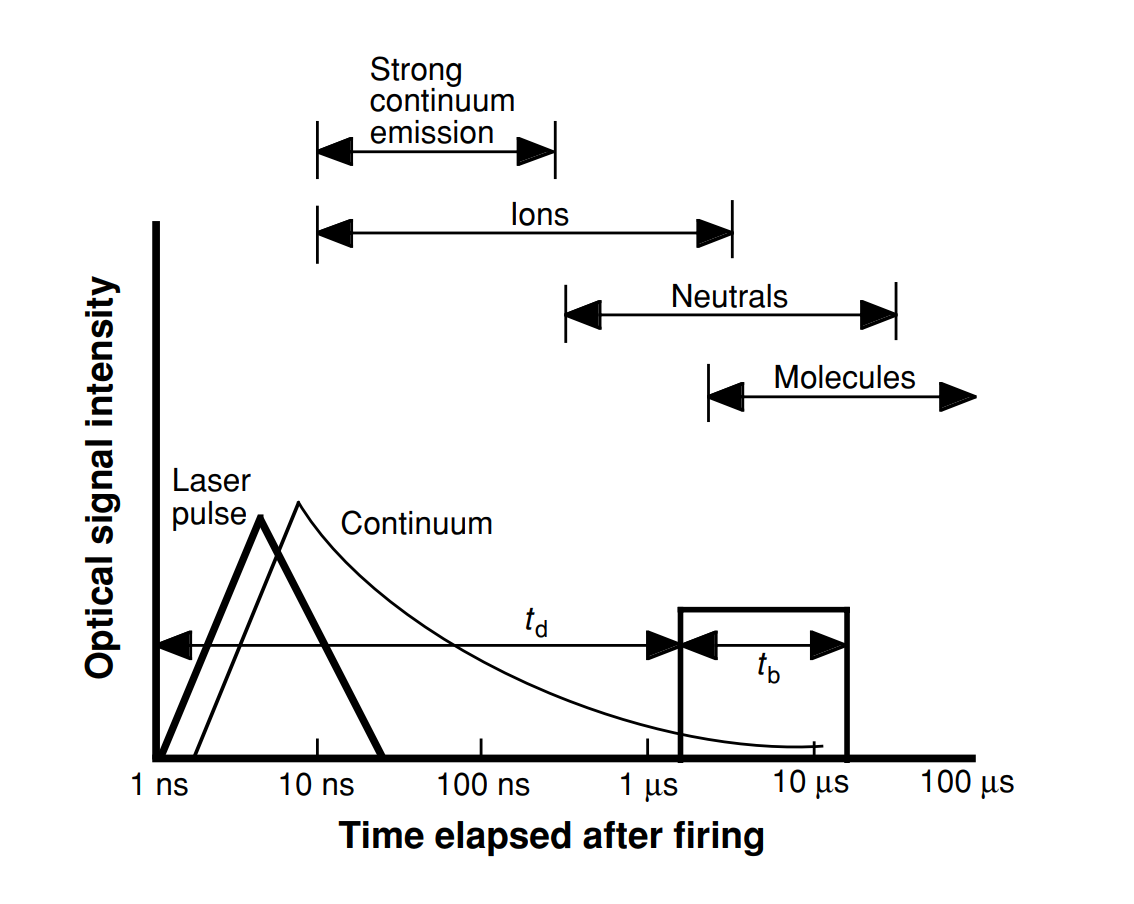
\includegraphics[width = \textwidth]{chapter_1/time_plasma_emission.png}
    \caption{Evolution of the emission of the LIBS plasma over time.}
    \label{fig:time_plasma_emission}
\end{figure}

\subsubsection{Plasma Parameters and Emission Characteristics}
\label{subsubsec:plasma_parameters}
Bound-to-bound transitions are characterized by a fixed energy value, equal to the energy difference between the initial and final level. However, experimentally we see that the measured emission spectrum is not constituted by a collection of sharp lines, but of bell curves instead, with different FWHM. This is because spectral line profiles are also influenced by broadening mechanisms; specifically, pure Doppler broadening, caused by the thermal movement of the emitting particles, will lead to a Gaussian profile, while natural line broadening, due to the time-energy uncertainty principle, and collision broadening will lead to a Lorentzian profile. The collisions between ions and electrons will result in Stark broadening due to the presence of high intensity electric fields near the particles; this phenomenon is predominant in plasmas with higher electron densities, due to the higher probability of collision. 
\\
The Stark broadening causes energy levels to be split according to the value of the quantum number $m_j$, associated with the $z$ component of the total angular momentum $J$, resulting in an asymmetric broadening.
The overall line shape depends on the relative intensity of the different broadening mechanisms and will have a resulting profile obtained by the convolution of the Gaussian and Lorentzian curves, called a Voigt profile.

\begin{figure}[H]
    \centering
    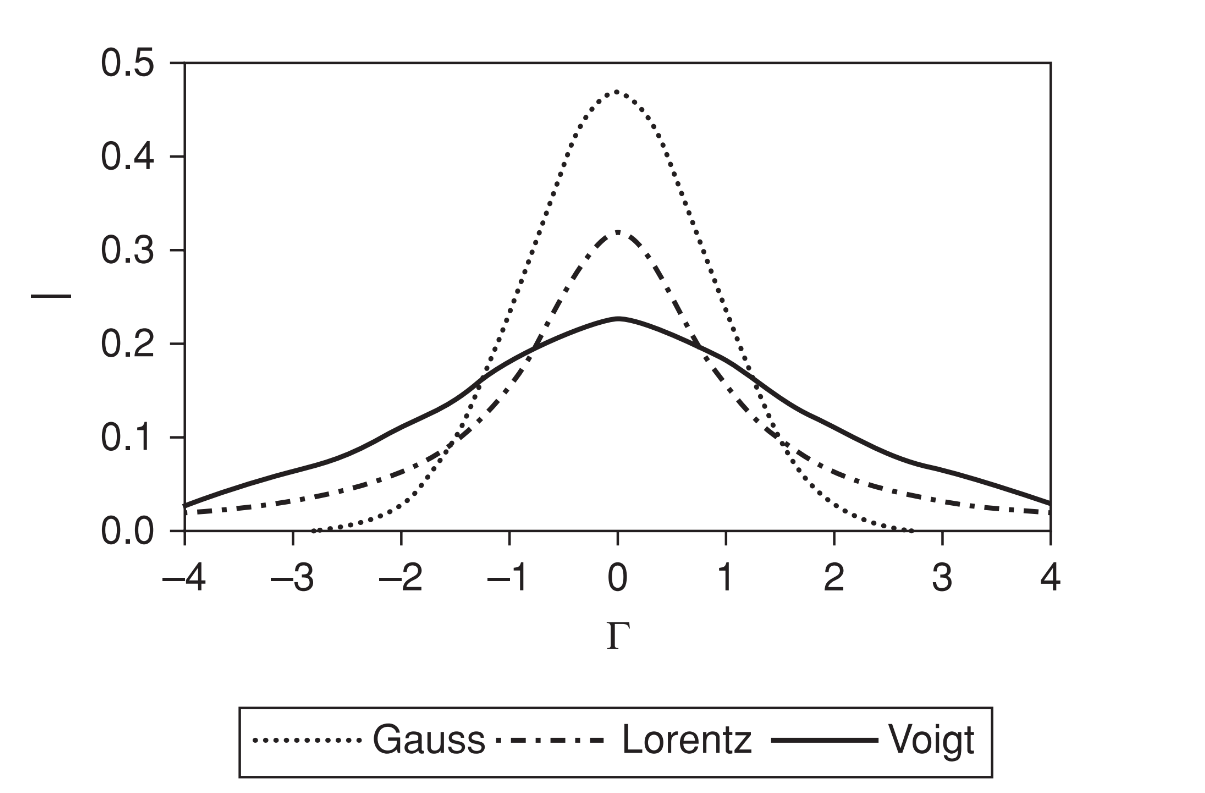
\includegraphics[width = 0.6\textwidth]{chapter_1/voigt.png}
    \caption{Plot of a Voigt profile.}
    \label{fig:voigt}
\end{figure}
[taken from https://scipython.com/book/chapter-8-scipy/examples/the-voigt-profile/]
\\
In normal conditions the main contributions of broadening in a LIBS plasma are due to Doppler and Stark effect. Natural line width is always present but usually the effect is so small that, even without the presence of other broadening mechanisms, it would not be resolved by commonly used LIBS spectrometer ($\Delta\lambda = 0.002\:nm$ for a $10\:ns$ transition at $500\:nm$).
\\
The Doppler width depends only on the temperature of the plasma and on the mass of the particles that are emitting the electromagnetic waves:
\begin{align}
    \Delta\lambda_{D}=7.2\times{10}^{-7}\left(T/M\right)^{1/2}\lambda_{o} \label{eq:doppler_eq}
\end{align}

The Stark effect will produce both a broadening and a shift, and both are dependent on the electron density ($N_e$) and can be used experimentally to obtain the parameter:

\begin{align}
    w_{\mathrm{total}}&\sim\left[1+1.75A\left(1-0.75r\right)\right]\left(n_{e}/{10}^{16}\right)w \label{eq:stark_width} \\ 
    d_{\mathrm{total}}&\sim\left[d/w+2.00A\left(1-0.75r\right)\right]\left(n_{e}/{10}^{16}\right)w \label{eq:stark_shift} 
\end{align}

\subsubsection{Plasma Opacity}
\label{subsubsec:plasma_opacity}
A plasma is defined as “optically thin” when the emitted radiation can freely escape from the plasma without being absorbed or scattered. This is a crucial characteristic to have in a plasma used for LIBS measurement, in this way the emitted radiation can be directly and more easily correlated with the atomic concentrations in the material.
\\
In general, the intensity of the radiation is given by:

\begin{align}
  I\left(\lambda\right)=\left[\varepsilon\left(\lambda\right)/\alpha\left(\lambda\right)\right]\left[1-\exp{\left(-\alpha\left(\lambda\right)L\right)}\right] \label{eq:intensity_radiation}  
\end{align}

Where $\varepsilon$ is the emissivity, $\alpha$ is the absorption coefficient and L is the plasma length in the direction of the observer. For an optically thin plasma we have that $\alpha$ is small and therefore:

\begin{align}
   I(\lambda)=[\varepsilon(\lambda)/\alpha(\lambda)][\alpha(\lambda)L]\varepsilon(\lambda)L \label{eq:intensity_radiation_approx}  
\end{align}

For strong lines, self-absorption will manifest as a flat-topped profile while for other cases certain lines will appear to have a dip in the middle of the curve, in that case the line is called “self-reversed”. 

\begin{figure}[H]
    \centering
    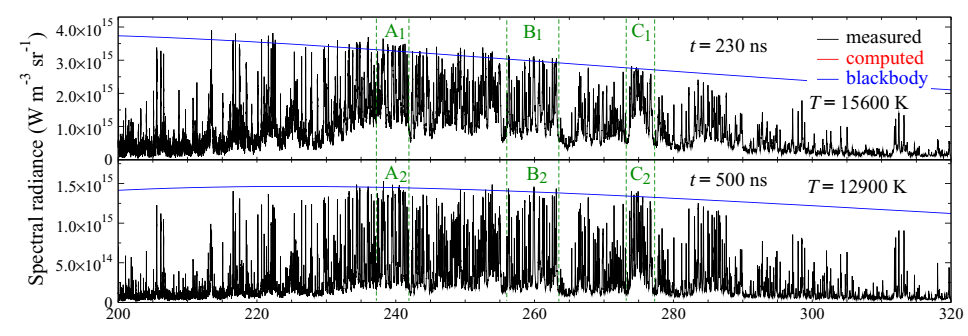
\includegraphics[width = \textwidth]{chapter_1/self_absorption_flat.png}
    \caption{Flat-topped profile of a spectrum caused by self-absorption.}
    \label{fig:self_absorbed_flat}
\end{figure}

\begin{figure}[H]
    \centering
    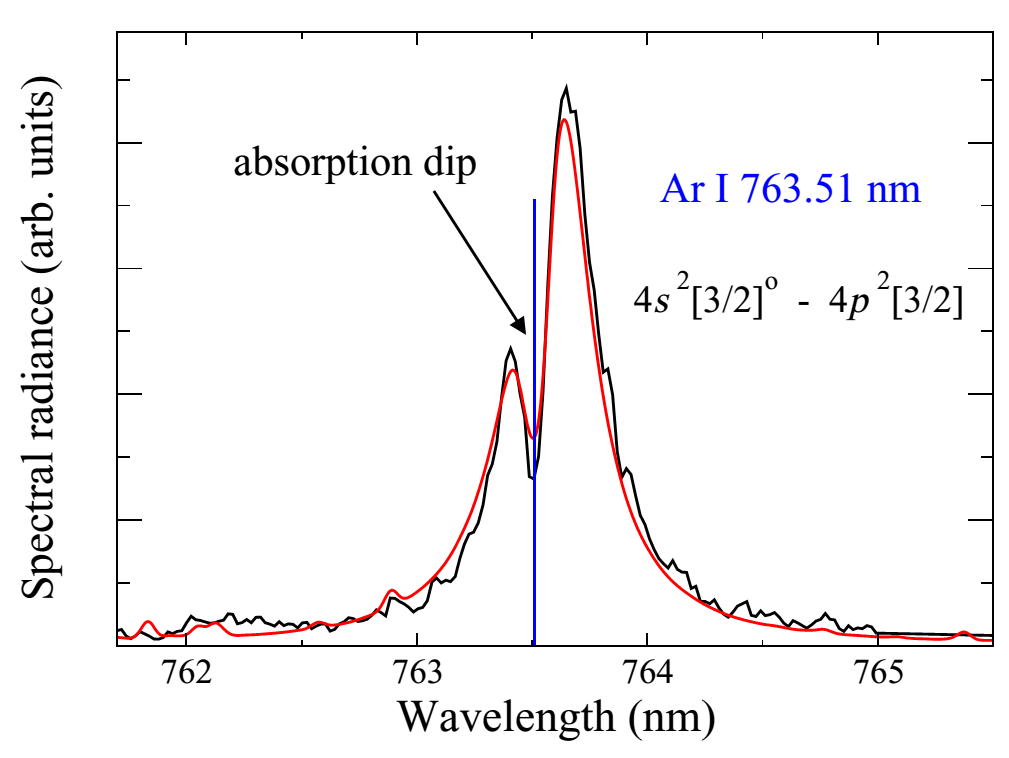
\includegraphics[width = 0.8\textwidth]{chapter_1/self_absorption_peak.png}
    \caption{Self-reversed line caused by high optical thickness.}
    \label{fig:self_absorbed_peak}
\end{figure}
[Taken from jorg's powerpoint]

\subsubsection{Thermodynamic Equilibrium and Plasma Temperature}
\label{subsubsec:thermodynamic_eq}

If a plasma is in thermodynamic equilibrium, it means that all the individual species (electrons, ions, atoms, and molecules) can be described by the same temperature. This condition is generally not true; collisions between particles of the same mass have a much higher probability of equally distributing the kinetic energy after the interaction, this leads to the different species achieving equilibrium individually but not globally, and in general the plasma will be characterized by a different temperature for each one of them.

\begin{figure}[H]
    \centering
    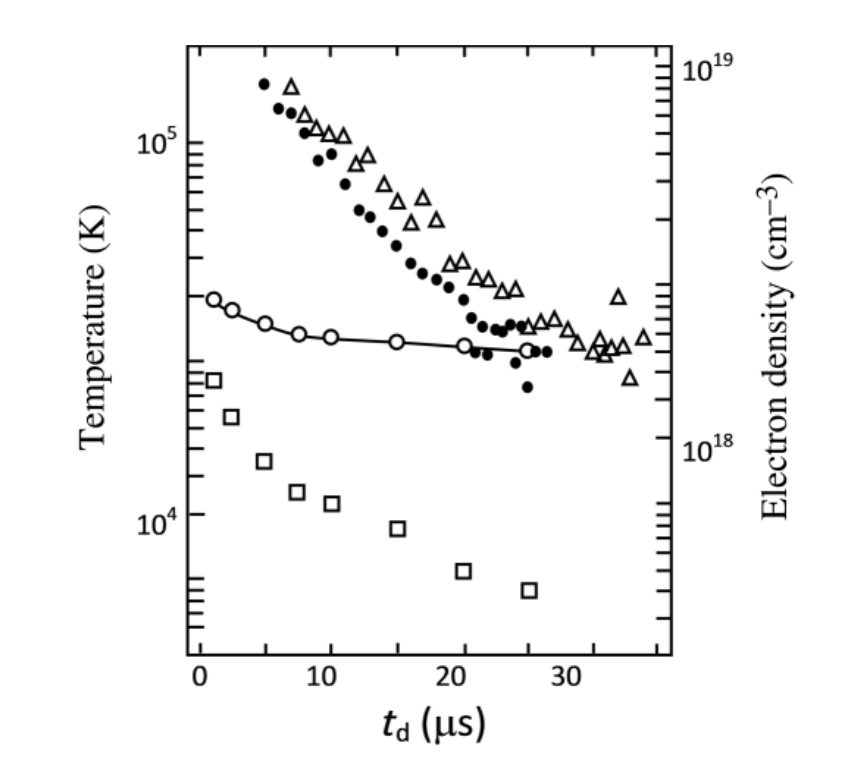
\includegraphics[width = 0.8\textwidth]{chapter_1/electron_equilibrium.png}
    \caption{Convergence of electron temperature for an air plasma.}
    \label{fig:electron_equilibrium}
\end{figure}
[taken from the HANDBOOK of libs]\\
In Figure~\ref{fig:electron_equilibrium} we can see electrons reaching global equilibrium $25\:\mu s$ after the incidence of the pulse. By looking at the Figure~\ref{fig:time_plasma_emission} is evident that the intensity of the emission decays exponentially, and at $25\: \mu s$ the magnitude is already negligible. For this reason, the condition of global thermodynamic equilibrium is not usually required, and it is enough to demand the “Local Thermodynamic Equilibrium” (LTE), where we assume that the equilibrium is reached only locally in small portions of the plasma.
\\
An important criterion to test if a plasma is in thermodynamic equilibrium is the so-called “McWhirter criterion”; is used to see if the electron density is high enough for collision to dominate the population of levels. 
\\
The McWhirter criterion can be expressed by this relation: 

\begin{align}
   n_{e}>1.6\times{10}^{12}T^{1/2}\left(\Delta E\right)^3 \label{eq:mcwhirter_criterion}  
\end{align}
Where $\delta E$ is the energy of the first level above the ground state.
\\
A more precise way to check if the LTE condition is valid is to see if the plasma respects the theoretical temperatures calculated by the Boltzmann and Saha equations. 
For $N_o$ electrons distributed between two levels $i,j$ with respective populations $N_i$ and $N_j$, the relative population will be given by the Boltzmann distribution:
\begin{align}
   N_j/N_{o}=\left(g_j/Z\right)\exp{\left[-E_j/kT\right]}N_j/N_i=\left(g_j/g_i\right)\exp{\left[-\left(E_j-E_i\right)/kT\right]} \label{eq:boltzmann_distribution}  
\end{align}
Where $g_{i,j}$ are the statistical weights and $Z$ is the partition function.
\\
The spectral radial intensity for a given transition with an energy $\lambda$ is then given by: 

\begin{align}
   I=hvAN/4\pi=\left(hcN_0gA/4\pi\lambda Z\right)\exp{\left[-E/kT\right]} \label{eq:spectral_radial_int}  
\end{align}
Where A is the transition probability (Einstein coefficient).
\\
A better and more reliable way to measure the temperature is to use more than one line simultaneously and perform an analysis graphically. By rearranging the previous expression, we obtain:
\begin{align}
   \ln{\left(I\lambda/gA\right)}=-E/kT-\ln{\left(4\pi Z/hcN_0\right)} \label{eq:bolzmann_plot_eq}  
\end{align}

In this way there is a linear dependence between the logarithm of a parameter related to the line intensity and the transition energy, with an angular coefficient $1/kT$. By plotting various transitions of the same element, if the data follows a linear trend, the assumption of LTE is valid, and it is possible to obtain the temperature from the slope.

\begin{figure}[H]
    \centering
    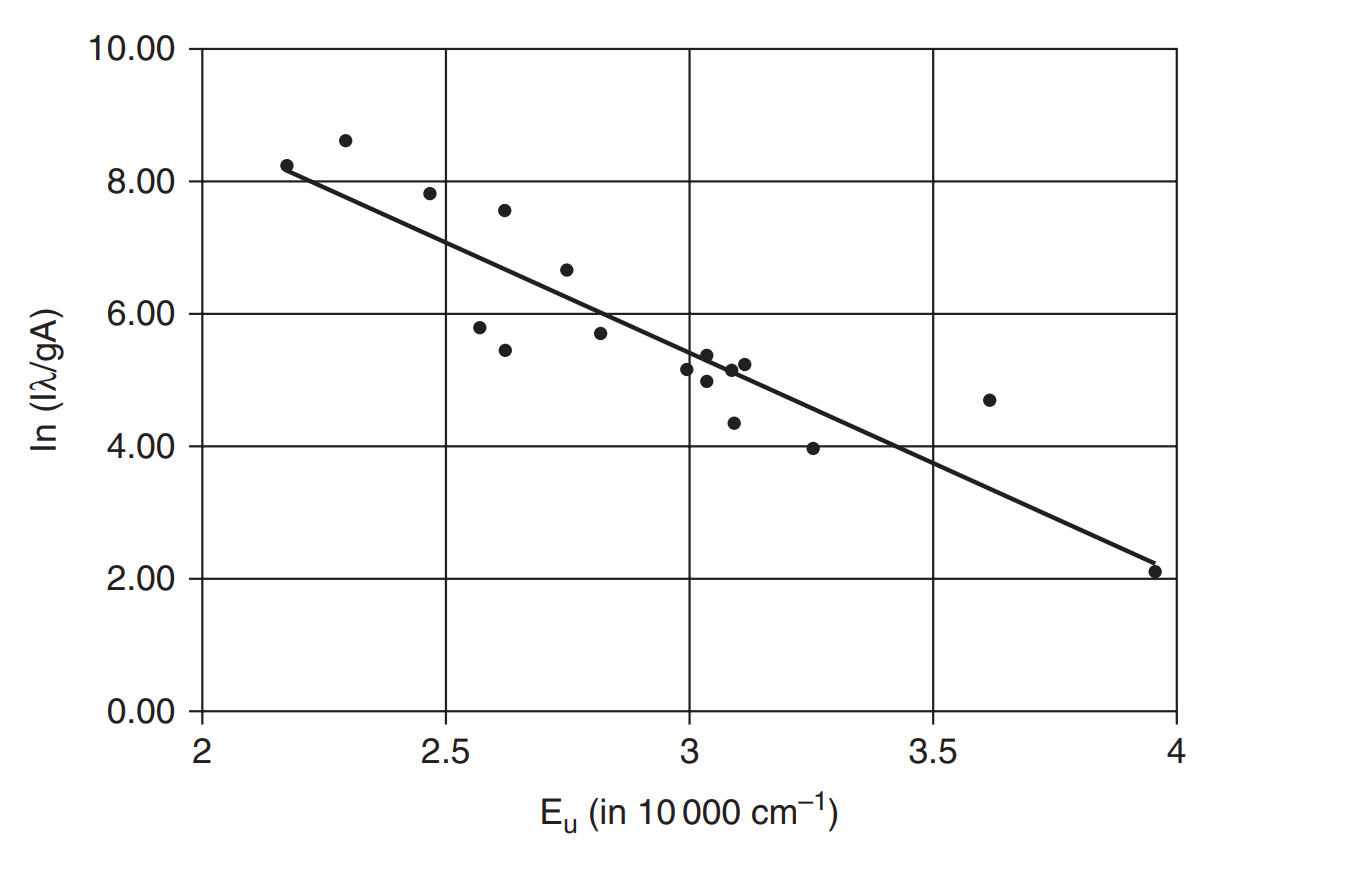
\includegraphics[width = 0.7\textwidth]{chapter_1/boltzmann_plot.png}
    \caption{Multi-line Boltzmann plot based on uranium data.}
    \label{fig:boltzmann_plot_example}
\end{figure}
[taken from the HANDBOOK of libs]\\
While the Boltzmann equation regulates the different populations of energy levels in neutral atoms and molecules, the Saha equation describes the relative populations of different ion stages of a certain atomic species in LTE. The expression of the equation is:

\begin{align}
   \frac{N\left(Z,0\right)}{N\left(Z-1,0\right)}n_{e}=\left(2\left(2\pi m k T\right)^{3/2}/h^3\right)\left(gA\left(Z,0\right)/gA\left(Z-1,0\right)\right)\exp{\left[-\Delta E/kT\right]} \label{eq:saha_equation}  
\end{align}

Where $N(Z,0)$ and $N(Z-1,0)$ represent the population of the ground state of the ion stages $Z$ and $Z-1$ respectively and $\Delta E$ is the ionization energy. It is important to underline that in this case the electron density must be known to apply the expression.
\\
Both equations can be used in conjunction to test for LTE and to estimate the temperature.

\subsection{LIBS Setup Components}
\label{subsec:libs_setup_component}
[taken from Fundamentals and applications]
In a LIBS analysis, four main devices are involved:
\begin{enumerate}
    \item High-energy pulsed laser: Typically operating with nanosecond-duration pulses, the laser is directed at the sample that needs to be studied, causing surface evaporation, and inducing plasma formation.
    \item Spectrometer: Responsible for both diffracting the light collected through an appropriate optical system to obtain its spectral signature and then detecting the intensity of the light at each wavelength. This can be achieved using various devices such as photomultiplier tubes (PMT), photodiode arrays (PDA), or charge-coupled devices (CCD). 
    \item Computer: Processes the acquired spectrum, allowing for further analysis.
\end{enumerate}

Precise time control is crucial in LIBS applications, plasma undergoes various stages in its lifetime that need to be managed to improve the spectral signature.
\\
The selection of the laser, combined with the spectrometer, detector, and time control unit, must be adapted according to the surrounding environmental conditions and the type of materials to analyze.

\subsubsection{Laser}
\label{subsubsec:laser_setup_component}
The laser is the central component of the LIBS system, providing the energy necessary to induce plasma formation. Consequently, the characteristics of the plasma are closely tied to the properties of the laser. The laser influence on the evolution of the plasma occurs both during the interaction between the laser pulse and the sample surface and during the interaction of the laser pulse with the generated plasma plume.
\\
The main parameters related to the laser source include:
\begin{itemize}
    \item Wavelength.
    \item Pulse energy.
    \item Pulse duration (typically in the nanosecond range).
    \item Repetition rate (number of pulses per second) or pulses per measurement.    
\end{itemize}

\paragraph{Wavelength}
\label{par:wavelength_setup_component}
After the initiation of the ablation process, the laser pulse interacts with the gas plume composed of ablated material from the sample's surface. As previously discussed, when the energy of the incoming photon exceeds the bond energy of the electron, photoionization occurs.
\\
Plasma formation primarily occurs through two processes: inverse bremsstrahlung and photoionization. In inverse bremsstrahlung, free electrons gain kinetic energy by absorbing photons from the incident laser light during collisions with atoms and ions.
\\
Inverse bremsstrahlung is more favorable for infrared (IR) and longer wavelengths. [Fundamentals and applications, 26] Consequently, laser sources with shorter wavelengths transfer energy to the material more efficiently, leading to higher ablation rates since the effect of plasma shielding is lower. However, for the same reason plasma ignition is less efficient with shorter wavelengths, resulting in a higher threshold for plasma formation. On the other hand, longer wavelengths will transfer energy to the plasma more efficiently but resulting in lower surface ablation.
\\
A variety of lasers are utilized in LIBS systems, with solid-state Nd: YAG lasers being commonly employed. This choice is attributed to their relatively low cost, ease of maintenance, and compact size, enabling their integration into systems of various sizes. The Nd: YAG laser typically operates at a fundamental wavelength of $1064\:nm$ with a pulse temporal width between $6$ and $15\:ns$. However, it is common for these lasers to operate at higher harmonics, such as the second harmonic at $532\:nm$, the third harmonic at $355\:nm$, or the fourth harmonic at $266\:nm$. These higher harmonics are less powerful and feature shorter pulse durations, typically between 4 and $8\:ns$ [Fundamentals and Applications].

\paragraph{Pulse Energy}
\label{par:pulse_energy_setup_component}
Both ablation and plasma ignition are significantly influenced by the energy and temporal duration of the laser pulse. In LIBS applications, the energy delivered to the sample per unit area is a more critical parameter than the absolute energy value of the laser pulse. Therefore, the primary physical quantities used in the analysis are Fluence, which represents energy per unit area (measured in $J/cm^2$), and Irradiance, which represents power per unit area (measured in $W/cm^2$).
\\
For this reason, fluence and irradiance can be adjusted both by varying the energy of the pulse and by tuning the focal length of the system, in order to change the spot size of the laser on the sample surface.
\\
Variations in pulse energies and focusing distances will also impact the shape and temporal evolution of the plasma plume [Analytical Chemistry LIBS]. At high irradiances, the plasma will contain more ablated material and possess greater internal energy, allowing it to expand with a hemispherical shape by pushing the surrounding air farther away. Conversely, at lower fluence levels, the plume will expand with less energy, resulting in a shape similar to a disk that evolves radially and remains closer to the surface of the sample.
\paragraph{Laser Pulse Duration}
\label{par:laser_pulse_duration_setup_component}

Regardless of their duration, laser pulses typically meet the necessary conditions for ablating targets. The rate of energy deposition will, indeed, surpass the rate of energy redistribution and dissipation through the sample lattice, leading to extremely high temperatures in those regions where energy absorption occurs.
\\
The nature of ablation is strongly influenced by the duration of the laser pulse.
When using lasers that generate pulses in the femtosecond regime, non-thermal processes dominate the ionization. This means that since the pulse duration is too short to induce thermal effects in the sample's matrix structure, other mechanisms are therefore responsible for ionizing the atoms. In this case, the pulse carries a significant amount of energy, and phenomena such as photochemical absorption, multi-photon absorption, tunneling, and avalanche ionization occur to excite the sample. 
\\
The absence of thermal effects results in the formation of a crater with sharply defined edges, without any melted or deposited materials surrounding it. After the laser pulse, only a very hot electron gas and an essentially undisturbed lattice remain.
\\
Conversely, when using laser pulses in the nanosecond regime, different effects come into play. The time required for electron-lattice heating is approximately $1\:ps$ [Fundamentals and Applications], much shorter than the duration of the pulse. As a result, thermal effects dominate the ionization process.
\\
After the interaction with the laser pulse, the material undergoes transient changes in thermodynamic states, transitioning from solid to liquid and ultimately into a plasma state [Analytical Chemistry].
\\
In simple terms, the pulse initially melts and vaporizes the surface, with the increasing temperature eventually leading to the ionization of atoms. If the irradiance is sufficiently high, both thermal and non-thermal effects will contribute to the ionization of the sample. Between 1 and $10 \: ns$, the plasma becomes opaque to laser radiation [Fundamentals and Applications]. As a result, the latter part of the pulse does not significantly contribute to surface vaporization. Instead, it interacts with the already generated plasma plume, potentially being absorbed, or reflected. This interaction leads to a decrease in the ablation rate, a phenomenon known as "Plasma Shielding." 
\\
Plasma Shielding is highly dependent on environmental conditions such as pressure and the composition of gases in the atmosphere, as well as experimental factors including laser wavelength and irradiance.
\\
When using nanosecond pulses, the generated craters typically exhibit melted and deposited material around them, as seen in the SEM images shown in Figure~\ref{fig:craters_laser_duration}:
\begin{figure}[H]
    \centering
    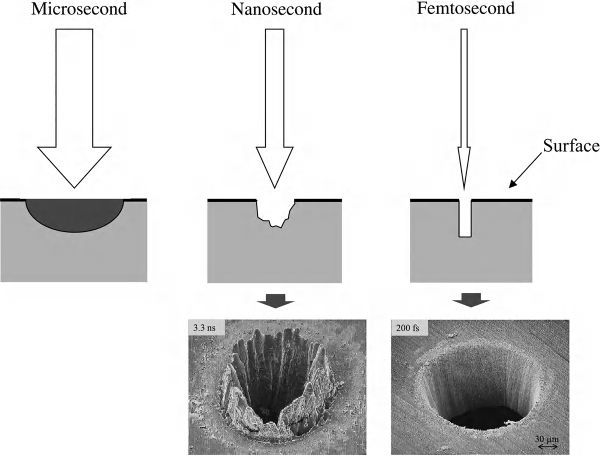
\includegraphics[width = 0.7\textwidth]{chapter_1/craters_laser_duration.jpg}
    \caption{SEM images of craters produced by different types of laser.}
    \label{fig:craters_laser_duration}
\end{figure}
[taken from the HANDBOOK of LIBS]
\\
At the same time, the plasma is reheated, resulting in longer plasma lifetimes and larger plasma plume sizes [Fundamentals and Applications].
\subsection{Spectra Evaluation}
\label{subsec:spectra_evaluation}
Once the plasma has been ignited, the emitted light is collected by a detector, which creates a spectrum with the intensities of the measured light on the $y$ axis, and the wavelengths on the $x$ axis. 
\begin{figure}[H]
    \centering
    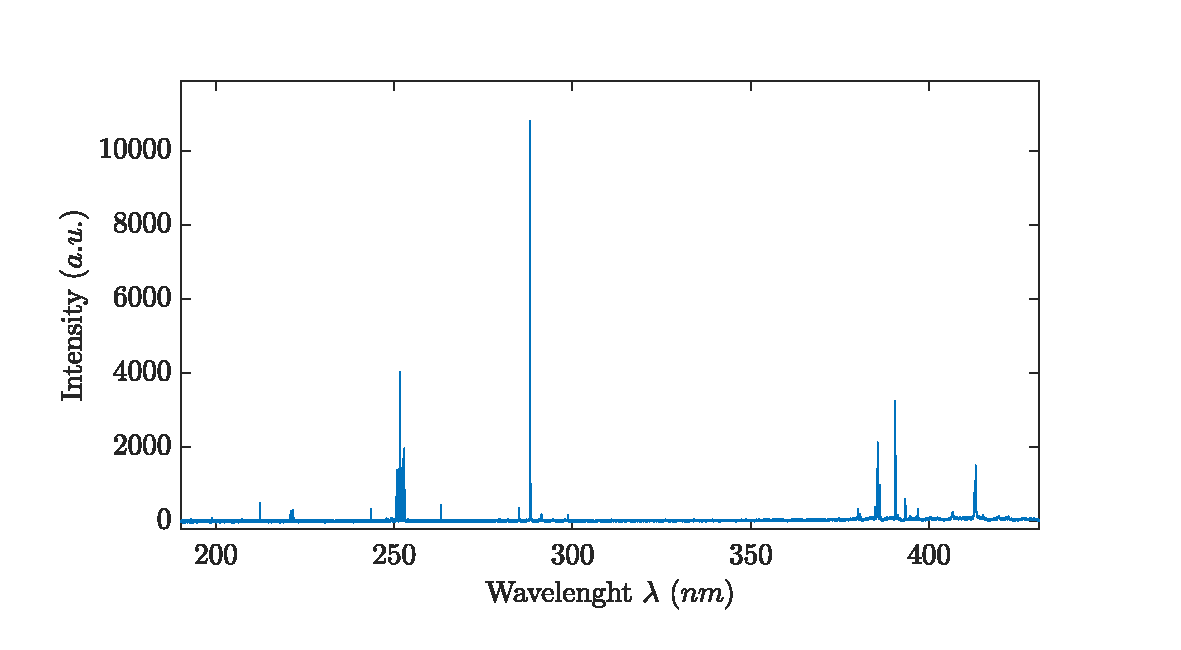
\includegraphics[width = \textwidth]{chapter_1/generic_spectrum.pdf}
    \vspace*{-30pt}
    \caption{LIBS spectrum of a pure silica sample we measured.}
    \label{fig:generic_spectrum}
\end{figure}
This spectrum may contain emission lines from atomic species, as well as continuous radiation resulting from bremsstrahlung [Fundamentals and Applications].
\\
Continuous radiation can hide emission lines, so efforts should be made to minimize its detection. 
\\
Since the energy of a transition is characteristic of the particle species, analyzing photon energies can reveal the composition of the plasma.
Accurate identification of LIBS emission lines is essential for determining the elemental constituents of a sample. The analysis of the LIBS spectrum will reveal elements present at concentrations above the method's minimum detectable limit (LOD).
\\
The most important spectral region for LIBS typically spans from 200 to $800\: nm$, where most elements exhibit strong emission lines. In addition to emission from atoms and ions, emission from simple molecules may also be observed in the samples. Generally, high concentrations of the elements composing the molecules must be present for molecular emission to be observed.
\\
Currently, LIBS is limited by problems of low reproducibility, with a resulting poor accuracy. Problems associated whit shot to shot variations in plasma conditions, which are caused by the stochastic nature of the laser source and light-matter interaction, seem to be the major cause of this effect [Applications of single-shot laser]. For this reason, a single measurement is usually obtained by averaging hundreds of different shots.
\\
More details on spectra evaluation will be presented in %Chapter~\ref{}